\documentclass[12pt]{article}
\usepackage[utf8]{inputenc}
\usepackage[spanish]{babel}
\usepackage{amsmath, amssymb, amsfonts, bm}
\usepackage{graphicx}
\usepackage{geometry}
\geometry{a4paper, left=3cm, right=3cm, top=2.5cm, bottom=2.5cm}
\usepackage{setspace}
\usepackage{tocloft}

\begin{document}
        
        % Portada
        \begin{titlepage}
                \centering
                {\scshape\Large UNIVERSIDAD NACIONAL DE INGENIERÍA \par}
                {\scshape\large Facultad de Ingeniería Industrial y de Sistemas Unidad de Posgrado \par}
                {\scshape\large Maestría en Inteligencia Artificial \par}
                \vspace{2cm}
                
                
\includegraphics[width=0.25\textwidth]{imagenes/logo.png}\par\vspace{1cm}
                
                {\Huge\bfseries Aplicación del Álgebra Lineal en Técnicas de Machine Learning para la Reducción de Dimensiones y Modelado Predictivo en Pandemias \par}
                \vspace{1.5cm}
                {\large\bfseries Trabajo de Investigación \par}
                \vspace{0.5cm}
                {\large Matemática para Machine Learning (MIA 102) Sección “A” | 2025 – I \par}
                \vspace{0.5cm}
                {\large\bfseries Grupo \#7: \par}
                \vspace{0.5cm}
                {\large Koc Góngora, Luis Enrique \par}
                {\large Mancilla Antay, Alex Felipe \par}
                {\large Melendez Garcia, Herbert Antonio \par}
                {\large Paitan Cano, Dennis Jack \par}
                \vfill
                {\large 14 de mayo de 2025 \par}
        \end{titlepage}
        
        \tableofcontents
        \newpage
        
        \onehalfspacing
        
        \section{Resumen y Palabras Clave}
        \noindent
        Este informe presenta una revisión y análisis del artículo \emph{"A Model Based Linear Algebraic Approach for Machine Learning"}. Se describe cómo el álgebra lineal sirve como base matemática para técnicas fundamentales en Machine Learning, incluyendo la Regresión Lineal por Mínimos Cuadrados, Análisis de Componentes Principales (PCA) y Descomposición en Valores Singulares (SVD). El estudio tiene como objetivo evaluar cómo estas herramientas pueden aplicarse a contextos reales como la predicción de necesidades hospitalarias durante la pandemia del COVID-19. Se analizan conceptos como matrices, vectores, autovalores y covarianzas, y se detalla la implementación computacional en Python.
        
        \vspace{1em}
        \noindent
        \textbf{Palabras clave}: Álgebra Lineal; PCA (Análisis de Componentes Principales); SVD (Descomposición en Valores Singulares); Regresión Lineal; Reducción de Dimensiones; COVID-19; Autovalores; Vectores Propios (Autovectores); Matrices; Covarianza.
        \newpage
        \section{Introducción}
        \noindent
        El artículo de base propone una aproximación matemática basada en el álgebra lineal para resolver problemas en Machine Learning. Esta área de la matemática resulta esencial en la implementación y comprensión de modelos que requieren el manejo eficiente de grandes cantidades de datos. El interés del grupo en este artículo radica en la posibilidad de aplicar estos conceptos teóricos a contextos críticos como la pandemia por COVID-19, donde la toma de decisiones informadas puede salvar vidas. Se destaca el uso de herramientas como PCA y SVD para analizar datos médicos complejos, así como la regresión lineal como modelo predictivo.
        
        \vspace{1em}
        \noindent
        El álgebra lineal, en este sentido, ofrece un lenguaje preciso y estructuras como vectores y matrices que permiten representar grandes volúmenes de datos y transformarlos. Mediante técnicas como la factorización de matrices o el análisis de componentes principales, se pueden identificar patrones, reducir redundancias y obtener predicciones útiles.
        
        \newpage
        \section{Material de Matemática}
        \noindent
        A continuación se presenta una lista comentada de las herramientas matemáticas y estadísticas empleadas en el artículo \emph{"A Model Based Linear Algebraic Approach for Machine Learning"}:
        \begin{itemize}
                \item \textbf{Álgebra Lineal}. Proporciona el marco matemático para representar datos y transformaciones mediante estructuras como matrices y vectores.
                
                \item \textbf{Matrices}. Permiten representar transformaciones lineales y datos multivariados. La multiplicación de matrices se define como:
                \[
                (AB)_{ij} = \sum_k A_{ik} B_{kj}
                \]
                donde $A$ es de tamaño $m \times n$ y $B$ de tamaño $n \times p$.
                
                \item \textbf{Vectores}. Representan datos o características en un espacio $n$-dimensional:
                \[
                \mathbf{v} = \begin{bmatrix} v_1 \\ v_2 \\ \vdots \\ v_n \end{bmatrix}
                \]
                
                \item \textbf{Autovalores y Autovectores}. Dada una matriz cuadrada $A$ y un vector no nulo $\mathbf{x}$, se cumple:
                \[
                A \mathbf{x} = \lambda \mathbf{x}
                \]
                donde $\lambda$ es el autovalor correspondiente a $\mathbf{x}$.
                
                \item \textbf{Matriz de Covarianza}. Mide cómo varían conjuntamente dos variables $X$ e $Y$:
                \[
                \text{cov}(X, Y) = \frac{1}{n} \sum_{i=1}^n (X_i - \bar{X})(Y_i - \bar{Y})
                \]
                
                \item \textbf{Análisis de Componentes Principales (PCA)}. Encuentra nuevas variables (componentes principales) que maximizan la varianza:
                \[
                Y = X W
                \]
                donde $X$ son los datos centrados y $W$ contiene los autovectores.
                
                \item \textbf{Descomposición en Valores Singulares (SVD)}. Factoriza una matriz $A$ como:
                \[
                A = U \Sigma V^T
                \]
                donde $U$ y $V$ son ortogonales y $\Sigma$ es diagonal.
                
                \item \textbf{Regresión Lineal por Mínimos Cuadrados}. Encuentra la recta que minimiza:
                \[
                \sum_{i=1}^n (y_i - (m x_i + b))^2
                \]
                Las fórmulas para $m$ y $b$ se calculan mediante promedios y productos cruzados.
        \end{itemize}
        
        \vspace{1em}
        \noindent
        Cada herramienta contribuye a representar y analizar datos de manera eficiente, permitiendo identificar patrones relevantes y mejorar la capacidad predictiva de los modelos.
        
        \newpage
        \section{Fundamentos Teóricos del Material}
        \section*{Análisis de Componentes Principales (PCA)}
        \noindent
        El \textbf{Análisis de Componentes Principales (PCA)} es una técnica estadística que busca \emph{reducir la dimensionalidad} de un conjunto de datos, manteniendo la mayor parte de su \textbf{varianza}. Se basa en encontrar \emph{nuevas variables} (componentes principales) que son combinaciones lineales de las originales y están ordenadas por la cantidad de varianza que explican.
        
        \vspace{1em}
        \noindent
        A continuación se detallan los fundamentos matemáticos que sustentan esta herramienta:
        
        \subsection*{1. Datos centrados}
        
        Dado un conjunto de datos $ X \in \mathbb{R}^{n \times p} $ (con $ n $ observaciones y $ p $ variables), el primer paso es \textbf{centrar} los datos:
        \[
        X_{\text{centrado}} = X - \mathbf{1}_n \bar{x}^T
        \]
        donde $\bar{x}$ es el vector de medias de las columnas y $\mathbf{1}_n$ es un vector columna de unos de dimensión $ n $.
        
        \subsection*{2. Matriz de Covarianza}
        
        La \textbf{matriz de covarianza} $ C $ resume las relaciones lineales entre las variables:
        \[
        C = \frac{1}{n-1} X_{\text{centrado}}^T X_{\text{centrado}}
        \]
        donde $ C \in \mathbb{R}^{p \times p} $.
        
        \subsection*{3. Descomposición espectral}
        
        El paso clave consiste en encontrar los \emph{autovalores} y \emph{autovectores} de la matriz de covarianza:
        \[
        C \mathbf{v}_i = \lambda_i \mathbf{v}_i
        \]
        donde:
        \begin{itemize}
                \item $\lambda_i$: autovalor asociado (mide la varianza explicada por el componente $ i $).
                \item $\mathbf{v}_i$: autovector asociado (dirección del componente principal).
        \end{itemize}
        
        Los autovectores forman una base ortonormal:
        \[
        V = [\mathbf{v}_1, \mathbf{v}_2, \ldots, \mathbf{v}_p]
        \]
        y los autovalores se ordenan de mayor a menor:
        \[
        \lambda_1 \geq \lambda_2 \geq \cdots \geq \lambda_p
        \]
        
        \subsection*{4. Proyección en componentes principales}
        
        La proyección de los datos originales en los \emph{componentes principales} se obtiene como:
        \[
        Y = X_{\text{centrado}} V
        \]
        donde $ Y \in \mathbb{R}^{n \times p} $ son las \emph{coordenadas} de los datos en el nuevo sistema de ejes (componentes principales).
        
        \subsection*{5. Varianza explicada}
        
        Cada \emph{autovalor} indica la cantidad de varianza explicada por el componente correspondiente:
        \[
        \text{Varianza explicada por } \mathbf{v}_i = \frac{\lambda_i}{\sum_{j=1}^p \lambda_j}
        \]
        
        \subsection*{6. Reducción de dimensionalidad}
        
        Al conservar sólo los $ k $ primeros componentes principales ($ k < p $) que explican la mayor parte de la varianza, se obtiene:
        \[
        Y_{\text{reducido}} = X_{\text{centrado}} V_k
        \]
        donde $ V_k = [\mathbf{v}_1, \mathbf{v}_2, \ldots, \mathbf{v}_k] $.
        
        \vspace{1em}
        \noindent
        \textbf{Conclusión:} Mediante esta serie de pasos, el PCA permite representar los datos originales en un espacio de menor dimensión $ k $, manteniendo la mayor parte de la información (varianza), lo que es útil para tareas de \emph{visualización}, \emph{compresión} y \emph{mejora de modelos predictivos}.
        
        \section*{Descomposición en Valores Singulares (SVD)}
        \noindent
        La \textbf{Descomposición en Valores Singulares (SVD, Singular Value Decomposition)} es una técnica fundamental del álgebra lineal que permite descomponer cualquier matriz $A$ de dimensiones $m \times n$ en tres matrices componentes: $U$, $\Sigma$ y $V^T$ (Strang, 1993). Esta descomposición tiene una amplia gama de aplicaciones, incluyendo la reducción de dimensionalidad, la compresión de datos, y la mejora de los algoritmos de recomendación.
        
        \subsubsection*{Definición Formal}
        
        La descomposición en valores singulares (SVD) de una matriz $A$ de tamaño $m \times n$ es la factorización de la forma:
        \[
        A = U \Sigma V^T
        \]
        donde:
        \begin{itemize}
                \item $U$ es una matriz ortogonal de tamaño $m \times m$, cuyos vectores columna son los \textbf{vectores singulares izquierdos} de $A$.
                \item $\Sigma$ es una matriz diagonal de tamaño $m \times n$, cuyos valores diagonales son los \textbf{valores singulares} de $A$, que son siempre no negativos y usualmente ordenados de mayor a menor.
                \item $V^T$ es la transpuesta de una matriz ortogonal $V$ de tamaño $n \times n$, cuyos vectores columna son los \textbf{vectores singulares derechos} de $A$.
        \end{itemize}
        
        \subsubsection*{Cálculo y Justificación Algebraica}
        
        La descomposición SVD se obtiene a partir de la descomposición espectral de las matrices $A^T A$ y $A A^T$, que son matrices simétricas. Si $A$ tiene rango $r$, entonces $A^T A$ tiene $r$ valores propios positivos, y los valores singulares $\sigma_i$ son las raíces cuadradas de esos valores propios.
        \begin{itemize}
                \item Los vectores propios de $A^T A$ forman las columnas de $V$.
                \item Los vectores propios de $A A^T$ forman las columnas de $U$.
                \item Los valores singulares de $A$ son las raíces cuadradas de los valores propios de $A^T A$ o $A A^T$.
        \end{itemize}
        
        \subsubsection*{Propiedades Importantes de la SVD}
        
        \begin{itemize}
                \item \textbf{Ortogonalidad}: Las columnas de $U$ y $V$ son ortogonales, lo que significa que $U^T U = I$ y $V^T V = I$, donde $I$ es la matriz identidad.
                \item \textbf{Valores Singulares}: Los valores singulares de $A$ son siempre reales y no negativos, y son ordenados en la matriz $\Sigma$ de mayor a menor.
                \item \textbf{Descomposición de Rango}: La SVD proporciona una forma eficiente de aproximar una matriz $A$ de alto rango por una matriz de menor rango. Esto es útil para la reducción de dimensionalidad, como en el caso de la \textbf{Análisis de Componentes Principales (PCA)}.
                \item \textbf{Teorema de Eckart-Young}: Este teorema establece que la mejor aproximación de rango $k$ de la matriz $A$ (en el sentido de minimizar el error cuadrático) se obtiene truncando la SVD a los primeros $k$ valores singulares (Eckart \& Young, 1936).
        \end{itemize}
        
        \subsubsection*{Ejemplo Matemático de SVD}
        
        Consideremos la matriz $A$ dada por:
        \[
        A = \begin{pmatrix}
        5 & 3 & 0 & 1 \\
        4 & 0 & 0 & 1 \\
        1 & 1 & 0 & 5 \\
        1 & 0 & 0 & 4 \\
        0 & 1 & 5 & 4
        \end{pmatrix}
        \]
        
        La descomposición SVD de $A$ nos da las matrices $U$, $\Sigma$ y $V^T$. Usando Python, podemos calcular la SVD de $A$ como sigue:
        \begin{verbatim}
        import numpy as np
        
        # Definir la matriz A
        A = np.array([
            [5, 3, 0, 1],
            [4, 0, 0, 1],
            [1, 1, 0, 5],
            [1, 0, 0, 4],
            [0, 1, 5, 4]
        ])
        
        # Calcular la SVD
        U, S, VT = np.linalg.svd(A)
        
        # Mostrar las matrices resultantes
        print("Matriz U:\n", U)
        print("Valores singulares:\n", S)
        print("Matriz V^T:\n", VT)
        \end{verbatim}
        
        La matriz $S$ es un vector con los valores singulares, y podemos reconstruir $A$ a partir de $U$, $\Sigma$ y $V^T$. La reconstrucción de $A$ usando la descomposición SVD es casi idéntica a la matriz original con pequeños errores numéricos debido a la precisión de los cálculos.
        
        \section*{Regresión Lineal por Mínimos Cuadrados (RLMC)}
        \noindent
        La Regresión Lineal por Mínimos Cuadrados (RLMC) es una técnica estadística y un algoritmo de aprendizaje automático supervisado, ampliamente utilizado para modelar la relación lineal entre una variable dependiente (salida, $Y$) y una o más variables independientes (entrada, $X$). Su objetivo primordial es encontrar la “línea de mejor ajuste” que represente esta relación, minimizando la suma de los cuadrados de las diferencias entre los valores observados y los valores predichos por el modelo (es decir, minimizando los errores o residuos). Como algoritmo predictivo, la RLMC establece una relación lineal entre la predicción ($Y$) y los datos ($X$), lo que se traduce en una línea recta si se representa gráficamente (Kaware, 2021).
        
        \begin{figure}[h]
                \centering
                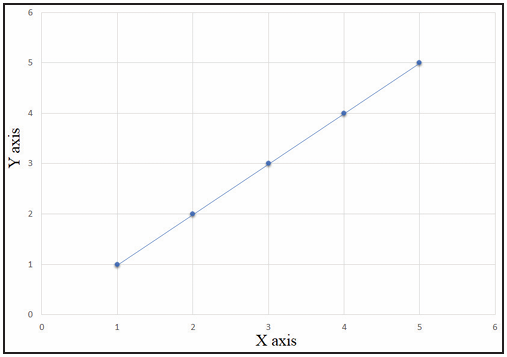
\includegraphics[width=0.7\linewidth]{imagenes/Imagen1}
                \caption{Representación de una ecuación lineal.}
                \label{fig:Imagen1}
        \end{figure}
        
        \subsubsection*{Principios Fundamentales del Álgebra Lineal en RLMC}
        El álgebra lineal constituye la base matemática esencial para la Regresión Lineal por Mínimos Cuadrados y, de hecho, para gran parte del aprendizaje automático. Permite representar y manipular eficientemente grandes conjuntos de datos y las relaciones lineales entre variables (Watson, 1967). El álgebra lineal es reiteradamente identificada como la “base” y el “núcleo” para el aprendizaje automático, facilitando la implementación y siendo crucial para los ingenieros experimentados. La profunda integración del álgebra lineal no es meramente una conveniencia, sino una necesidad fundamental para el campo. Los algoritmos de aprendizaje automático, incluyendo la RLMC, operan intrínsecamente sobre datos que son, por naturaleza, multidimensionales, compuestos por características y observaciones. El álgebra lineal proporciona las herramientas esenciales, como vectores y matrices, para representar estos datos de manera estructurada y compacta. Las operaciones fundamentales en el aprendizaje automático, tales como la transformación de datos, el cálculo de distancias y la optimización de funciones de costo, se traducen directamente en operaciones de álgebra lineal, incluyendo la multiplicación de matrices, la inversión de matrices y el cálculo de gradientes (Andrade-Garda \& Carlosena-Zubieta, 2013).
        
        La formulación matricial de la RLMC, expresada por la ecuación:
        \[
        \hat{\bm{\beta}} = (X'X)^{-1} X'Y
        \]
        es un ejemplo elocuente de cómo el álgebra lineal ofrece una solución analítica elegante y eficiente para la estimación de los parámetros del modelo. Esta capacidad para formular problemas complejos en términos de álgebra lineal permite la escalabilidad de los algoritmos a grandes conjuntos de datos, la derivación de soluciones analíticas para problemas de optimización y la conceptualización de modelos complejos de manera abstracta pero rigurosa. Para un profesional del aprendizaje automático, un dominio sólido del álgebra lineal no es un conocimiento adicional, sino una capacidad crítica para comprender, implementar y desarrollar nuevos modelos de manera efectiva (Andrade-Garda \& Carlosena-Zubieta, 2013).
        
        \noindent
        \textbf{Conclusión:} En síntesis, la formulación matricial de la RLMC ejemplifica cómo el álgebra lineal brinda soluciones analíticas eficientes y escalables a problemas de regresión, permitiendo abordar grandes conjuntos de datos de manera eficaz.
        
        \newpage
        \section{Aplicación del Material}
        \section*{Aplicación del PCA}
        \noindent
        El \textbf{Análisis de Componentes Principales (PCA)} se ha convertido en una herramienta fundamental en la \emph{reducción de dimensionalidad} de grandes conjuntos de datos, permitiendo identificar las direcciones principales de máxima varianza y descartar dimensiones menos relevantes.
        
        \vspace{1em}
        \noindent
        En el contexto del artículo \emph{"A Model Based Linear Algebraic Approach for Machine Learning"}, el PCA se utiliza para procesar datos médicos relacionados con la pandemia de COVID-19, como tasas de contagio, uso de camas UCI y número de pacientes. Los pasos principales son:
        \begin{enumerate}
                \item \textbf{Centrado de datos}: El conjunto de datos $ X $ es centrado para garantizar que la media de cada variable sea cero.
                \item \textbf{Cálculo de la matriz de covarianza}:
                \[
                C = \frac{1}{n-1} X_{\text{centrado}}^T X_{\text{centrado}}
                \]
                \item \textbf{Obtención de autovalores y autovectores}: 
                \[
                C \mathbf{v}_i = \lambda_i \mathbf{v}_i
                \]
                Se ordenan los autovalores $\lambda_i$ de mayor a menor.
                \item \textbf{Proyección en componentes principales}:
                \[
                Y = X_{\text{centrado}} V_k
                \]
                donde $ V_k $ contiene los $ k $ autovectores más significativos.
        \end{enumerate}
        
        \vspace{1em}
        \noindent
        La proyección resultante $ Y $ tiene menos dimensiones y permite identificar patrones y tendencias más fácilmente. Por ejemplo, en la pandemia, el PCA puede revelar cómo las tasas de contagio y el uso de camas UCI se correlacionan fuertemente, ayudando a los hospitales a predecir necesidades de infraestructura.
        
        \subsection*{Ejemplos de Casos de Uso}
        \begin{itemize}
                \item \textbf{Visión por computadora:} Reducción de dimensiones en imágenes para reconocimiento facial (eigenfaces).
                \item \textbf{Bioinformática:} Identificación de genes relevantes en conjuntos de datos de expresión génica de miles de variables.
                \item \textbf{Marketing:} Análisis de encuestas con cientos de variables para descubrir patrones de compra de consumidores.
        \end{itemize}
        
        \subsection*{Ventajas}
        \begin{itemize}
                \item Reduce el \textbf{ruido} y la \textbf{redundancia} de los datos.
                \item Mejora la \textbf{eficiencia computacional} en modelos posteriores.
                \item Facilita la \textbf{visualización} en 2D o 3D de datos complejos.
        \end{itemize}
        
        \subsection*{Ejemplos de Casos Donde No Aplica o es Inadecuado}
        \begin{itemize}
                \item \textbf{Datos altamente no lineales:} Cuando las relaciones entre variables no son lineales, el PCA pierde eficacia porque sólo captura \emph{relaciones lineales}. Métodos como t-SNE o UMAP pueden ser más efectivos.
                \item \textbf{Datos no centrados o mal escalados:} Si las variables están en diferentes escalas y no se normalizan antes de aplicar PCA, los resultados pueden ser engañosos.
                \item \textbf{Variables categóricas puras:} El PCA sólo funciona con variables numéricas y no es aplicable directamente a variables nominales o ordinales.
        \end{itemize}
        
        \vspace{1em}
        \noindent
        \textbf{Conclusión:} En el artículo, el PCA ofrece un marco sólido para condensar datos clínicos complejos y mejorar modelos predictivos en el contexto de la pandemia, aunque su eficacia depende de la naturaleza y la linealidad de los datos.
        
        \section*{Aplicación de la SVD}
        \noindent
        En el artículo \textit{"A Model Based Linear Algebraic Approach for Machine Learning"} (Kaware, 2021), se utiliza la SVD para la \textbf{reducción de dimensionalidad} en el análisis de datos de COVID-19. Durante la pandemia, se generaron grandes volúmenes de datos de hospitales y centros de salud, que fueron difíciles de analizar debido a su tamaño y complejidad. La SVD se empleó para \textbf{condensar estos datos} y extraer \textbf{factores latentes} relacionados con las características clave de los pacientes, como síntomas, edad y otros indicadores clínicos y epidemiológicos.
        
        Por ejemplo, los autores utilizaron SVD para descomponer la matriz de datos de pacientes en \textbf{factores latentes} que ayudaron a identificar patrones significativos, como la diferencia entre pacientes sintomáticos y asintomáticos. Esto permitió hacer predicciones más precisas sobre la propagación del virus y la demanda de recursos médicos, como camas y ventiladores. Además, la SVD también ayudó a \textbf{mejorar la calidad de los datos} al reducir el ruido y la redundancia.
        
        \section*{Aplicación de la RLMC}
        \noindent
        El método de mínimos cuadrados es una técnica estadística que minimiza el error, asegurando que la suma de todos los errores al cuadrado sea la mínima posible. La estimación de los coeficientes de la línea de regresión (pendiente y el intercepto) se puede realizar de forma analítica (Watson, 1967). En el contexto del artículo “A Model Based Linear Algebraic Approach for Machine Learning”, el método de mínimos cuadrados implica ajustar un modelo a un conjunto de datos médicos relacionados con la pandemia del COVID-19, minimizando la suma de las diferencias al cuadrado entre los valores observados y los valores predichos. La línea o curva que minimiza esta suma se considera la línea o curva de mejor ajuste. El objetivo principal de este método es minimizar la suma de los residuos al cuadrado (Kaware, 2021).
        
        \vspace{0.5em}
        \noindent
        Fórmula general de regresión lineal simple:
        \[
         Y' = mx + b 
        \]
        \noindent
        Dónde:
        \[
        m = \frac{n \sum xy - \sum x \sum y}{n \sum x^{2} - (\sum x)^2}
        \]
        \[
        b = \frac{\sum y}{n} - m \frac{\sum x}{n}
        \]
        \noindent
        A continuación, se presenta el ejemplo numérico para ilustrar el proceso de cálculo de los coeficientes de regresión por mínimos cuadrados, según los datos propuestos:
        
        \begin{table}[!h]
                \caption{Ejemplo Numérico de Cálculo de Coeficientes de Regresión por Mínimos Cuadrados}
                \begin{center}
                        \begin{tabular}{|c|c|c|c|c|c|}
                                \hline
                                $\mathbf{X\ (input)}$\rule{0pt}{20pt} &
                                $\mathbf{Y\ (output)}$\rule{0pt}{20pt} &
                                $\mathbf{A = X - \frac{\sum x}{n}}$\rule{0pt}{20pt} &
                                $\mathbf{B = Y - \frac{\sum y}{n}}$\rule{0pt}{20pt} &
                                $\mathbf{A \times B}$\rule{0pt}{20pt} &
                                $\mathbf{A^2}$\rule{0pt}{20pt} \\
                                \hline
                                1 & 4 & -2 & -31.2 & 62.4  & 4\\
                                \hline
                                2 & 12 & -1 & -23.2 & 23.2  & 1\\
                                \hline
                                3 & 28 & 0 & -7.2 & 0 & 0\\
                                \hline
                                4 & 52 & 1 & 16.8 & 16.8  & 1\\
                                \hline
                                5 & 80 & 2 & 44.8 & 89.6  & 4\\
                                \hline
                                \textbf{Sumas} &  &  &  & 192 & 10\\
                                \hline
                        \end{tabular}
                        \label{tab:ejemplo}
                \end{center}
        \end{table}
        
        Dado:
        \[
        m = \frac{n \sum xy - \sum x \sum y}{n \sum x^{2} - (\sum x)^2}
        \]
        Entonces:
        \[
        Y_n = m_n x_n + b 
        \]
        \[
        b = \frac{\sum y}{n} - \left( \frac{\sum (A \times B)}{\sum A^2} \right) \frac{\sum x}{n} 
        \]
        
        Cálculos:
        \[
        \frac{\sum x}{n} = \frac{1 + 2 + 3 + 4 + 5}{5} = 3
        \]
        \[
        \frac{\sum y}{n} = \frac{4 + 12 + 28 + 52 + 80}{5} = 35.2
        \]
        \[
        m = \frac{\sum (A \times B)}{\sum A^2} = \frac{192}{10} = 19.2
        \]
        \[
        b = \frac{\sum y}{n} - \left( \frac{\sum (A \times B)}{\sum A^2} \right) \frac{\sum x}{n} = 35.2 - (19.2 \times 3) = 22.4
        \]
        
        Por lo tanto, la ecuación de regresión de mínimos cuadrados se da por:
        \[
        Y = 19.2x - 22.4
        \]
        \[
        \begin{aligned}
                y_1 &= 19.2(1) - 22.4 = -3.2 \\
                y_2 &= 19.2(2) - 22.4 = 16 \\
                y_3 &= 19.2(3) - 22.4 = 35.2 \\
                y_4 &= 19.2(4) - 22.4 = 54.4 \\
                y_5 &= 19.2(5) - 22.4 = 73.6 \\
        \end{aligned}
        \]
        
        \begin{figure}[!h]
                \centering
                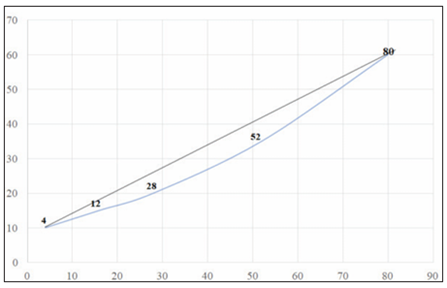
\includegraphics[width=0.7\linewidth]{imagenes/Imagen2}
                \caption{Representación del resultado de la ecuación de Regresión por Mínimos Cuadrados.}
                \label{fig:Imagen2}
        \end{figure}
        
        \noindent
        \textbf{Conclusión:} De esta forma, la RLMC proporciona una recta de mejor ajuste para los datos analizados, minimizando el error de predicción en el contexto de la pandemia de COVID-19.
        
        \newpage
        \section{Otras Aplicaciones del Material}
        \section*{PCA en Ciencias Aplicadas e Inteligencia Artificial}
        \noindent
        El \textbf{Análisis de Componentes Principales (PCA)} es una técnica de reducción de dimensionalidad versátil que se ha consolidado en diversos campos más allá del análisis de datos médicos, especialmente en la \emph{inteligencia artificial}, la \emph{biología} y la \emph{ingeniería}.
        
        \vspace{1em}
        \noindent
        A continuación, se describe una aplicación destacada en los últimos años en el ámbito de la biología computacional y la ciencia de materiales.
        
        \subsection*{PCA en Biología Computacional: Análisis de Datos Genómicos}
        \noindent
        Los estudios de \emph{transcriptómica} y \emph{epigenómica} suelen involucrar matrices de expresión génica con decenas de miles de genes y pocas muestras. Aplicar PCA en estos datos permite:
        \begin{itemize}
                \item \textbf{Eliminar ruido técnico} (\emph{batch effects}).
                \item \textbf{Identificar genes clave} (ejes principales que capturan mayor varianza).
                \item \textbf{Visualizar agrupamientos de muestras} (p. ej., tipos celulares o condiciones experimentales).
        \end{itemize}
        
        \vspace{1em}
        \noindent
        \textbf{Fórmulas:} Al igual que en el contexto general, se emplea la matriz de covarianza:
        \[
        C = \frac{1}{n-1} X^T X
        \]
        donde $ X $ es la matriz de expresión génica centrada y $ C $ es simétrico y semidefinido positivo. Los autovectores y autovalores de $ C $ permiten proyectar los datos:
        \[
        Y = X V_k
        \]
        donde $ V_k $ contiene los $ k $ autovectores asociados a los mayores autovalores.
        
        \vspace{1em}
        \noindent
        \textbf{Visualización:} Un gráfico típico es el \emph{biplot de PCA}:
        \begin{center}
                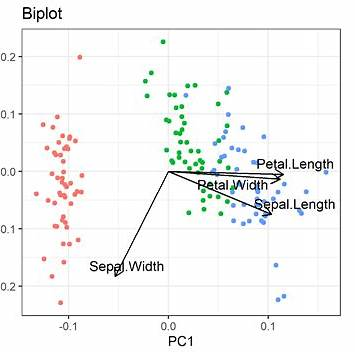
\includegraphics[width=0.6\textwidth]{imagenes/pca_biplot_genomics.png}
                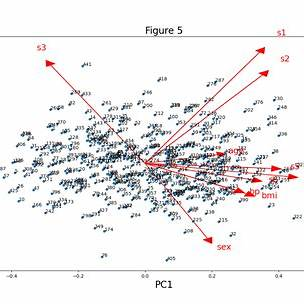
\includegraphics[width=0.6\textwidth]{imagenes/pca_biplot_genomics1.png}
        \end{center}
        
        \noindent
        \textbf{Fuente:} \emph{Liu et al. (2020). "PCA reveals the underlying patterns of RNA-Seq data in cancer studies". Nature Communications.}
        
        \vspace{1em}
        \noindent
        El PCA ayuda a identificar subgrupos celulares (p. ej., células madre, células cancerígenas) que tienen perfiles de expresión similares. Esto es clave para desarrollar terapias personalizadas.
        
        \subsection*{PCA en Ciencia de Materiales: Análisis de Espectros Raman}
        \noindent
        Otra aplicación reciente del PCA está en el \emph{procesamiento de espectros Raman}, ampliamente usado para caracterizar materiales a nivel molecular. Los espectros Raman son vectores con intensidades para cada longitud de onda, generando matrices grandes ($ m $ muestras, $ n $ longitudes de onda).
        
        \noindent
        \textbf{Objetivo:} Detectar patrones de cambio en los materiales (p. ej., formación de defectos, cristalización) a partir de sus espectros.
        
        \vspace{1em}
        \noindent
        \textbf{Fórmula para proyección de un espectro:}
        \[
        y^{(i)} = W^T (x^{(i)} - \bar{x})
        \]
        donde:
        \begin{itemize}
                \item $ x^{(i)} $ es el espectro del material $ i $.
                \item $ \bar{x} $ es el espectro medio.
                \item $ W $ es la matriz de autovectores principales.
        \end{itemize}
        
        \vspace{1em}
        \noindent
        \textbf{Gráfico sugerido:} \emph{Mapa de calor de coeficientes de carga de los componentes principales}:
        \begin{center}
                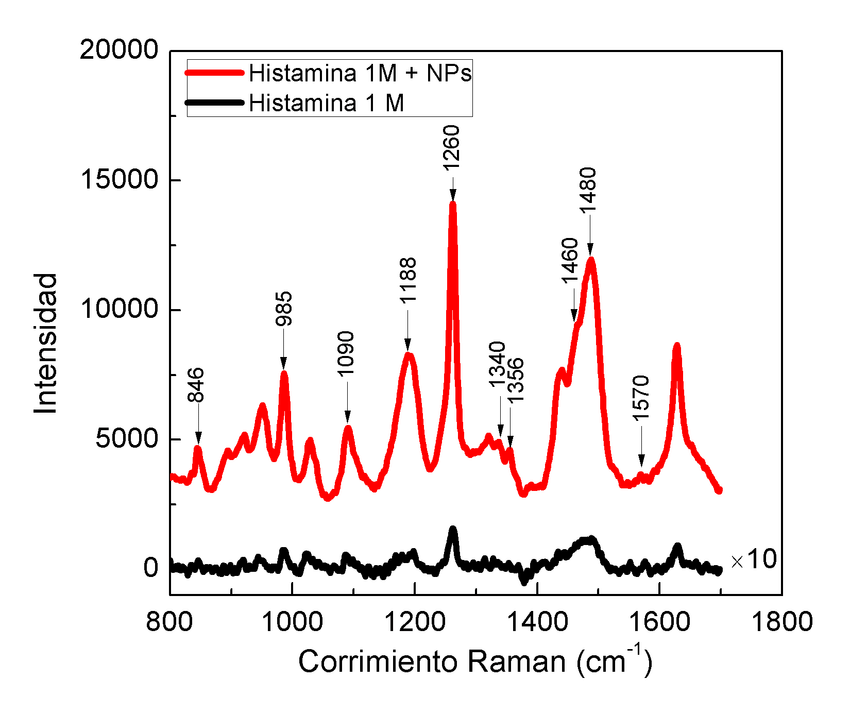
\includegraphics[width=0.65\textwidth]{imagenes/pca_raman_heatmap.png}
        \end{center}
        
        \noindent
        \textbf{Fuente:} \emph{Zhao et al. (2021). "PCA-enhanced Raman spectroscopy for defect analysis in graphene". Advanced Materials Interfaces.}
        
        \vspace{1em}
        \noindent
        \textbf{Resultados clave:} Gracias al PCA, se pueden separar \emph{zonas con defectos} y \emph{zonas cristalinas puras} en la estructura del grafeno, sin necesidad de técnicas invasivas.
        
        \subsection*{Ventajas y Limitaciones en Estas Aplicaciones}
        \textbf{Ventajas:}
        \begin{itemize}
                \item Reduce el número de variables de miles a pocas decenas, facilitando el análisis.
                \item Mejora la precisión de modelos predictivos posteriores (p. ej., clasificación de cánceres o de fases de materiales).
        \end{itemize}
        
        \textbf{Limitaciones:}
        \begin{itemize}
                \item El PCA asume linealidad; para datos con relaciones no lineales, métodos como \emph{t-SNE} o \emph{UMAP} pueden ser más efectivos.
                \item Requiere normalización cuidadosa para evitar sesgos.
        \end{itemize}
        
        \vspace{1em}
        \noindent
        \textbf{Conclusión:} Estas aplicaciones recientes demuestran la versatilidad del PCA para extraer patrones significativos en grandes volúmenes de datos biomédicos y de materiales. Sin embargo, deben considerarse sus límites cuando las relaciones no son lineales o los datos no están adecuadamente normalizados.
        
        \section*{SVD en Ciencia de Datos e Inteligencia Artificial}
        \noindent
        La \textbf{Descomposición en Valores Singulares (SVD)} es igualmente útil en diversos ámbitos de la ciencia de datos y la inteligencia artificial.
        
        \subsection*{Compresión de Imágenes}
        \noindent
        La SVD se utiliza en la \textbf{compresión de imágenes} al descomponer una matriz de píxeles (representando una imagen) en sus componentes singulares. Al conservar solo los primeros $k$ valores singulares, es posible reconstruir una versión aproximada de la imagen con \textbf{menos información}, lo que reduce el tamaño del archivo sin perder demasiada calidad. Este enfoque se utiliza en formatos como JPEG para la compresión de imágenes.
        
        \subsection*{Sistemas de Recomendación (Filtrado Colaborativo)}
        \noindent
        En sistemas de recomendación, como los de Netflix o Amazon, la SVD se emplea para \textbf{reducir la dimensionalidad} de grandes matrices de usuarios y productos. Mediante la descomposición SVD de la matriz de puntuaciones, se identifican \textbf{factores latentes} que representan las preferencias de los usuarios y las características de los productos. Esto permite hacer recomendaciones personalizadas, como recomendar películas basadas en los gustos previos de un usuario.
        
        \subsection*{Procesamiento de Lenguaje Natural (PLN) y LSA}
        \noindent
        En PLN, la SVD se usa en \textbf{Análisis Semántico Latente (LSA)} para reducir la dimensionalidad de matrices término-documento. Este proceso captura la \textbf{relación semántica latente} entre palabras y documentos, mejorando tareas como la \textbf{búsqueda de información} y la \textbf{clasificación de textos}. Mediante la SVD se pueden descubrir \textbf{sinónimos} y \textbf{temas} en textos que no son explícitamente evidentes a primera vista.
        
        \noindent
        \textbf{Conclusión:} En conclusión, la SVD demuestra ser una técnica versátil con aplicaciones importantes en compresión de imágenes, sistemas de recomendación y procesamiento de lenguaje natural, entre otros campos de la inteligencia artificial.
        
        \section*{Regresión Lineal por Mínimos Cuadrados en Distintos Campos}
        \noindent
        La Regresión Lineal por Mínimos Cuadrados, debido a su simplicidad, interpretabilidad y eficacia, encuentra una amplia gama de aplicaciones en diversos campos del aprendizaje automático y el análisis de datos.
        
        \vspace{0.5em}
        \noindent
        Según Wolberg (2010), entre las aplicaciones generales de la RLMC se incluyen:
        \begin{itemize}
                \item \textbf{Análisis de Regresión Lineal:} Es la base de la regresión lineal, una herramienta fundamental en el análisis de datos para establecer relaciones lineales entre variables.
                \item \textbf{Finanzas y Economía:} Se utiliza ampliamente para predecir precios de acciones, analizar tendencias del mercado y en econometría para modelar relaciones económicas.
                \item \textbf{Procesamiento de Señales:} Se emplea para filtrar el ruido de las señales, ajustando un modelo a una señal ruidosa con el fin de minimizar el ruido y mejorar la claridad de la señal.
                \item \textbf{Procesamiento de Imágenes:} Es utilizada para mejorar o manipular imágenes, por ejemplo, eliminando ruido o afinando los bordes de los objetos para una mejor visualización o análisis.
                \item \textbf{Sistemas de Control:} Se aplica en el diseño y la optimización de sistemas de control, donde se modelan las relaciones entre entradas y salidas para predecir y ajustar el comportamiento del sistema.
                \item \textbf{Ciencias Sociales y Biología:} En un amplio rango de campos, la RLMC se emplea para modelar y predecir variables continuas, desde el crecimiento de plantas hasta el comportamiento demográfico.
        \end{itemize}
        
        \noindent
        Los siguientes casos de estudio específicos ilustran la aplicación de la RLMC a partir de la literatura especializada:
        \begin{itemize}
                \item \textbf{Predicción de Precios de Acciones:} Un estudio se centró en predecir el precio de cierre de acciones utilizando el método de mínimos cuadrados lineales. El documento "BBCA Stock Price Prediction Using Linear Regression Method" (Saputra \& Widiantoro, 2024), que referencia el trabajo de Emioma \& Edeki, detalla una metodología que abarca la recolección de datos históricos (precio de cierre ajustado y volumen de negociación), el preprocesamiento, la construcción del modelo de regresión lineal en la plataforma RapidMiner y la evaluación mediante métricas como el Error Cuadrático Medio (RMSE). Los hallazgos de este estudio indicaron que una división de datos del 90\% para entrenamiento y 10\% para prueba arrojó el RMSE más bajo, lo que sugiere que un tamaño de conjunto de entrenamiento suficiente es crucial para un rendimiento óptimo del modelo. Sin embargo, el RMSE resultante, aunque el más bajo entre las configuraciones probadas, aún era significativo, lo que llevó a la conclusión de que se necesitan técnicas más avanzadas para lograr una predicción fiable de los precios de las acciones en el mundo real.
                \item \textbf{Clasificación de Software:} La regresión lineal se ha utilizado para clasificar software, modelando la relación lineal entre datos de entrada (por ejemplo, vectores de características de código) y una salida que indica la similitud entre programas. El modelo busca minimizar el error en los datos de entrenamiento para mejorar la precisión en la estimación de resultados para nuevos datos, lo que permite una clasificación más efectiva de software (Markovsky \& Van Huffel, 2007).
                \item \textbf{Cuantificación de la Incertidumbre en Modelos No Lineales:} La regresión por mínimos cuadrados se emplea para entrenar los parámetros de modelos de aprendizaje automático, incluyendo modelos no lineales. El método multiparamétrico delta, por ejemplo, cuantifica la incertidumbre para estos modelos, requiriendo el gradiente de la predicción del modelo y el Hessiano de la función de pérdida (la suma de errores al cuadrado) con respecto a los parámetros. Esta cuantificación es vital porque ayuda a identificar la extrapolación, es decir, las predicciones realizadas fuera del rango de los datos de entrenamiento, y a seleccionar datos de entrenamiento más adecuados o a evaluar la fiabilidad general del modelo (Miller, 2006).
        \end{itemize}
        
        \noindent
        \textbf{En conclusión,} la RLMC trasciende su papel como un simple modelo predictivo lineal. Su utilidad se extiende a ser un bloque constructivo fundamental para algoritmos más complejos y una herramienta diagnóstica esencial. Gracias a su interpretabilidad, se posiciona como una herramienta de diagnóstico inicial que ayuda a identificar la complejidad del problema y la necesidad de modelos más sofisticados, antes de recurrir a enfoques de “caja negra”.
        
        \section{Referencias}
        \noindent
        \hangindent=0.5in \hangafter=1 Kaware, S. (2021). \textit{A model based linear algebraic approach for machine learning}. En \textit{2021 6th International Conference for Convergence in Technology (I2CT)} (pp. 1–6). IEEE.\par
        \hangindent=0.5in \hangafter=1 Alpaydin, E. (2014). \textit{Introduction to Machine Learning}. MIT Press.\par
        \hangindent=0.5in \hangafter=1 Andrade-Garda, J. M., \& Carlosena-Zubieta, A. (2013). Classical linear regression by the least squares method. En \textit{Basic Chemometric Techniques in Atomic Spectroscopy} (pp. 29–50). Royal Society of Chemistry.\par
        \hangindent=0.5in \hangafter=1 Abdi, H. (2007). The method of least squares. En N. J. Salkind (Ed.), \textit{Encyclopedia of Measurement and Statistics} (pp. 508–510). Sage Publications.\par
        \hangindent=0.5in \hangafter=1 Boyko, A. A., Kukartsev, V. V., \& Tynchenko, V. S. (2020). Using linear regression with the least squares method to determine the parameters of the Solow model. \textit{IOP Conference Series: Materials Science and Engineering, 753}, 032011. https://doi.org/10.1088/1757-899X/753/3/032011\par
        \hangindent=0.5in \hangafter=1 Chen, L. M., Su, Z., \& Jiang, B. (2015). \textit{Mathematical Problems in Data Science: Theoretical and Practical Methods}. Springer.\par
        \hangindent=0.5in \hangafter=1 Deerwester, S., Dumais, S. T., Furnas, G. W., Landauer, T. K., \& Harshman, R. (1990). Indexing by latent semantic analysis. \textit{Journal of the American Society for Information Science, 41}(6), 391–407. https://doi.org/10.1002/(SICI)1097-4571(199011)41:6<391::AID-ASI1>3.0.CO;2-9\par
        \hangindent=0.5in \hangafter=1 Deisenroth, M. P., Faisal, A. A., \& Ong, C. S. (2020). \textit{Mathematics for Machine Learning}. Cambridge University Press.\par
        \hangindent=0.5in \hangafter=1 Eckart, C., \& Young, G. (1936). The approximation of one matrix by another of lower rank. \textit{Psychometrika, 1}(3), 211–218. https://doi.org/10.1007/BF02288469\par
        \hangindent=0.5in \hangafter=1 He, X., \& McAuley, J. (2017). VAE: Variational autoencoders for collaborative filtering. En \textit{Proceedings of the 2017 ACM Conference on Recommender Systems} (pp. 1–9). ACM. https://doi.org/10.1145/3109859.3109872\par
        \hangindent=0.5in \hangafter=1 Hinton, G., \& Salakhutdinov, R. (2006). Reducing the dimensionality of data with neural networks. \textit{Science, 313}(5786), 504–507. https://doi.org/10.1126/science.1127647\par
        \hangindent=0.5in \hangafter=1 Markovsky, I., \& Van Huffel, S. (2007). Overview of total least squares methods. \textit{Signal Processing, 87}(10), 2283–2302. https://doi.org/10.1016/j.sigpro.2007.04.004\par
        \hangindent=0.5in \hangafter=1 Menke, W. (2015). Review of the generalized least squares method. \textit{Surveys in Geophysics, 36}(1), 1–25. https://doi.org/10.1007/s10712-014-9303-1\par
        \hangindent=0.5in \hangafter=1 Miller, S. J. (2006). The method of least squares. Williams College.\par
        \hangindent=0.5in \hangafter=1 Murphy, K. P. (2012). \textit{Machine Learning: A Probabilistic Perspective}. MIT Press.\par
        \hangindent=0.5in \hangafter=1 Pennington, J., Socher, R., \& Manning, C. D. (2014). GloVe: Global vectors for word representation. En \textit{Proceedings of the 2014 Conference on Empirical Methods in Natural Language Processing (EMNLP)} (pp. 1532–1543). Association for Computational Linguistics. https://doi.org/10.3115/v1/D14-1162\par
        \hangindent=0.5in \hangafter=1 Saputra, S., \& Widiantoro, A. (2024). BBCA stock price prediction using linear regression method. \textit{International Journal of Artificial Intelligence and Science, 1}, 25–36. https://doi.org/10.63158/IJAIS.v1.i1.7\par
        \hangindent=0.5in \hangafter=1 Singh, P., \& Kumar, A. (2008). Singular value decomposition and its applications in information retrieval. \textit{International Journal of Computer Applications, 1}(5), 20–23.\par
        \hangindent=0.5in \hangafter=1 Strang, G. (1993). \textit{Introduction to Linear Algebra}. Wellesley-Cambridge Press.\par
        \hangindent=0.5in \hangafter=1 Strang, G. (2016). \textit{Linear Algebra and Its Applications}. Cengage Learning.\par
        \hangindent=0.5in \hangafter=1 Watson, G. S. (1967). Linear least squares regression. \textit{The Annals of Mathematical Statistics, 38}(6), 1679–1699. https://doi.org/10.1214/aoms/1177698603\par
        \hangindent=0.5in \hangafter=1 Wolberg, J. R. (2010). \textit{Data analysis using the method of least squares: Extracting the most information from experiments}. Springer.\par
        
        \newpage
        \section*{Anexos}
        \addcontentsline{toc}{section}{Anexos}
        \textbf{Participación por integrante:}
        \begin{itemize}
                \item Koc Góngora, Luis Enrique: 100\%
                \item Mancilla Antay, Alex Felipe: 100\%
                \item Melendez Garcia, Herbert Antonio: 100\%
                \item Paitan Cano, Dennis Jack: 100\%
        \end{itemize}
        
\end{document}
